\documentclass[a4paper]{article}

\usepackage{fullpage}

\usepackage{graphicx}
\usepackage{subcaption}

\usepackage{amsmath}
\usepackage{tabularx}

% Code for typesttting C code
\usepackage{listings}
\usepackage{color}

\definecolor{mygreen}{rgb}{0,0.6,0}
\definecolor{mygray}{rgb}{0.5,0.5,0.5}
\definecolor{mymauve}{rgb}{0.58,0,0.82}
\definecolor{mybrown}{rgb}{0.5,0,0}

\lstdefinestyle{MyCStyle}{ %
  language=C,                      % the language of the code
  backgroundcolor=\color{white},   % choose the background color; you must add \usepackage{color} or \usepackage{xcolor}
  basicstyle=\ttfamily    ,        % the size of the fonts that are used for the code
  breakatwhitespace=false,         % sets if automatic breaks should only happen at whitespace
  breaklines=true,                 % sets automatic line breaking
  captionpos=b,                    % sets the caption-position to bottom
  commentstyle=\color{mygreen},    % comment style
  deletekeywords={...},            % if you want to delete keywords from the given language
  escapeinside={\%*}{*)},          % if you want to add LaTeX within your code
  extendedchars=true,              % lets you use non-ASCII characters; for 8-bits encodings only, does not work with UTF-8
  frame=single,                    % adds a frame around the code
  keepspaces=true,                 % keeps spaces in text, useful for keeping indentation of code (possibly needs columns=flexible)
  keywordstyle=\color{blue},       % keyword style
  morecomment=[l][\color{mybrown}]\#,  % compiler directive
  morekeywords={*,...},            % if you want to add more keywords to the set
  numbers=left,                    % where to put the line-numbers; possible values are (none, left, right)
  numbersep=5pt,                   % how far the line-numbers are from the code
  numberstyle=\tiny\color{mygray}, % the style that is used for the line-numbers
  rulecolor=\color{black},         % if not set, the frame-color may be changed on line-breaks within not-black text (e.g. comments (green here))
  showspaces=false,                % show spaces everywhere adding particular underscores; it overrides 'showstringspaces'
  showstringspaces=false,          % underline spaces within strings only
  showtabs=false,                  % show tabs within strings adding particular underscores
  stepnumber=1,                    % the step between two line-numbers. If it's 1, each line will be numbered
  stringstyle=\color{mymauve},     % string literal style
  tabsize=2,                       % sets default tabsize to 2 spaces
  title=\lstname                   % show the filename of files included with \lstinputlisting; also try caption instead of title
}

\newlength{\pic}

\begin{document}

\title{EE445M Lab 7 Report}
\author{\bfseries Yen-Kai Huang, Siavash Zanganeh Kamali, Chen Cui, Miao Qi, Yan Zhang}
\maketitle

\section{Objective} This is the final robotic project. We build a robot and compete in the final race with other robots.

\section{Hardware Design}

\paragraph{(a) Final mechanical drawing of the robot }
See Figure-\ref{mech}

\setlength{\pic}{\textwidth}
\begin{figure}[htp]
\center
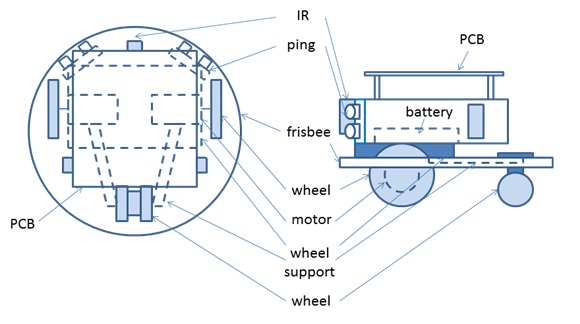
\includegraphics[width=\pic]{circuits/mechanical_drawing}
\caption{Mechanical Drawing} \label{mech}
\end{figure}

\paragraph{(b) Final electrical circuit diagram for the motor interfaces }
See Figure-\ref{pwm}

\setlength{\pic}{\textwidth}
\begin{figure}[htp]
\center
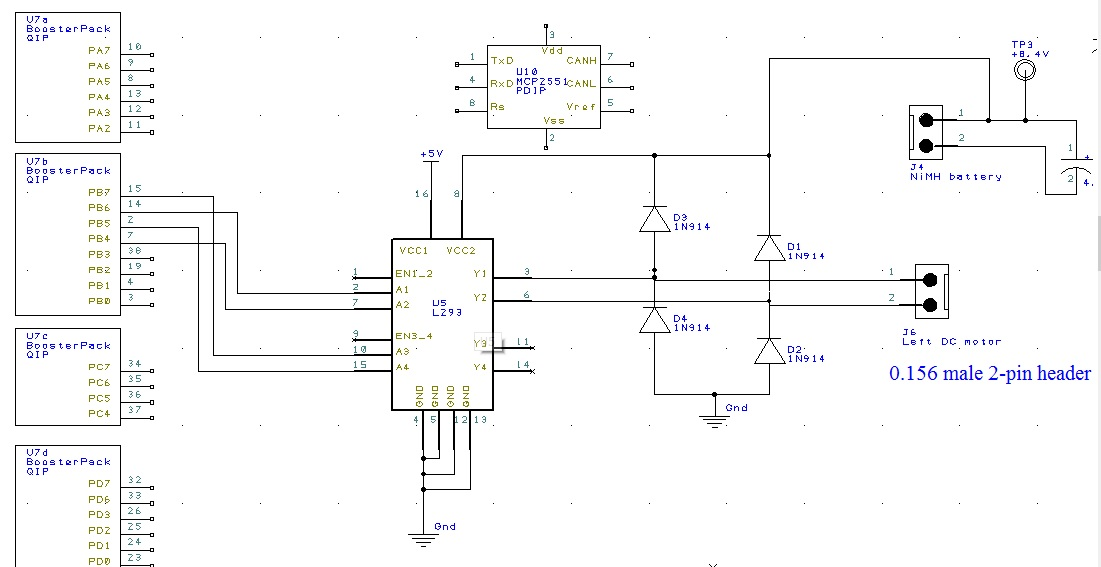
\includegraphics[width=\pic]{circuits/PWM_Circuit}
\caption{Motor Circuit} \label{pwm}
\end{figure}


\paragraph{(c) Final power supply circuitry }
See Figure-\ref{pw}

\setlength{\pic}{12cm}
\begin{figure}[htp]
\center
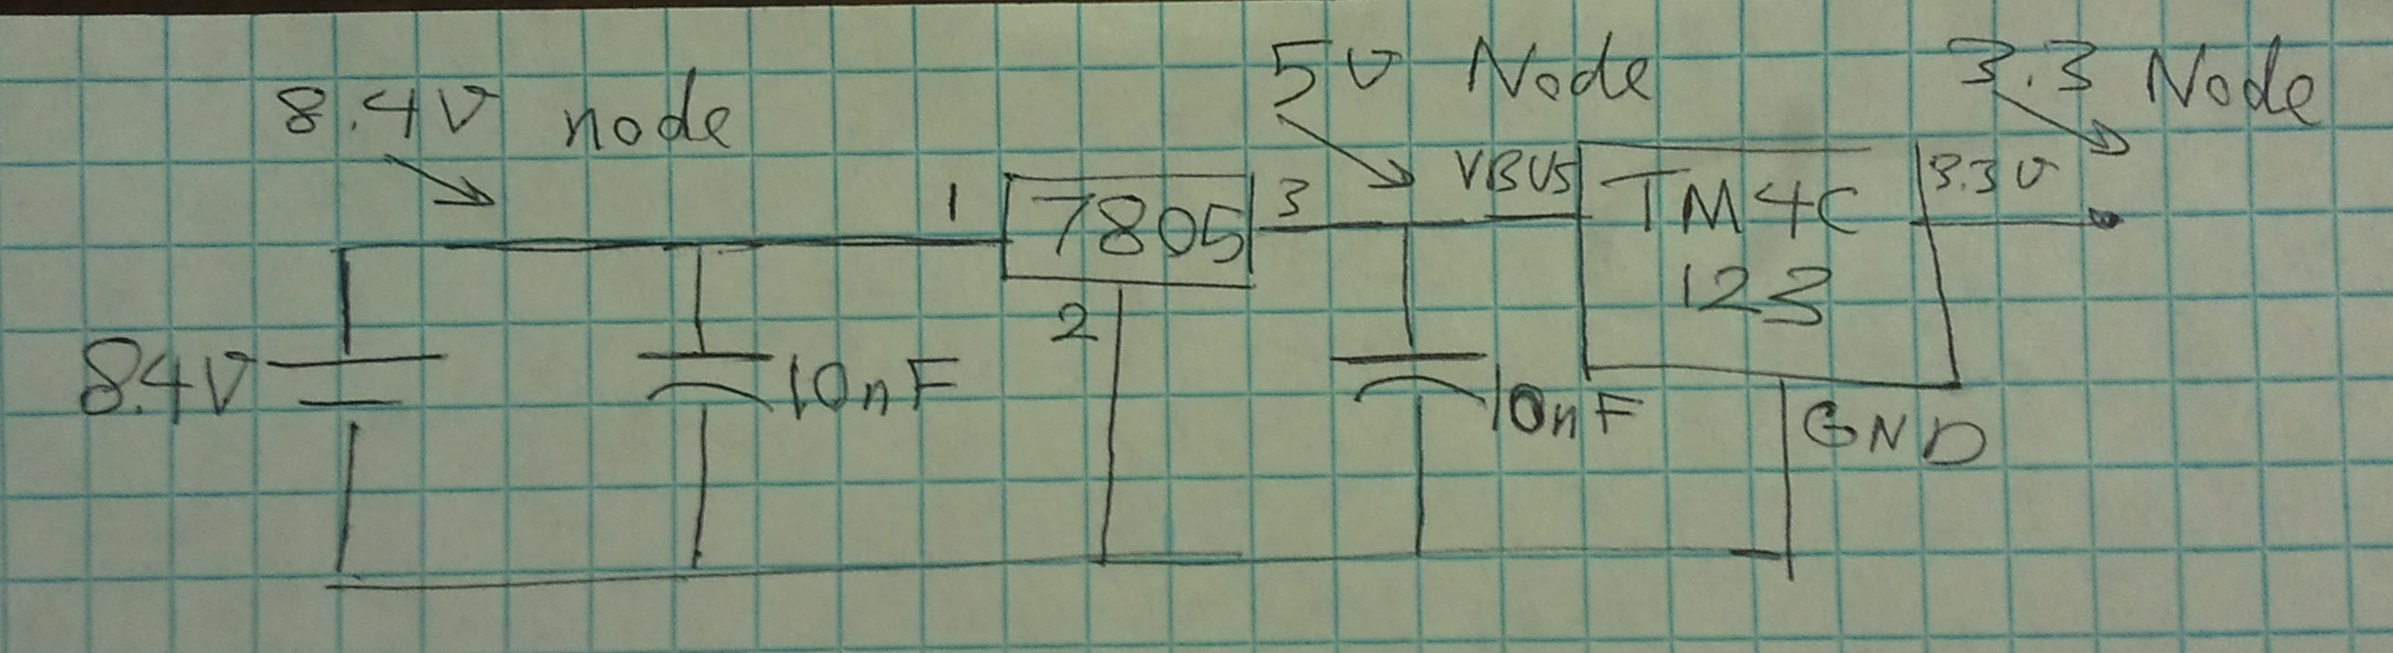
\includegraphics[width=\pic]{circuits/Power_Circuit}
\caption{Power Circuit} \label{pw}
\end{figure}


\paragraph{(d) Final electrical circuit diagram for the sensor interfaces \\}
See Figure-\ref{ping} for Ping circuits and Figure-\ref{ir} for IR sensor circuits.

\setlength{\pic}{12cm}
\begin{figure}[htp]
\center
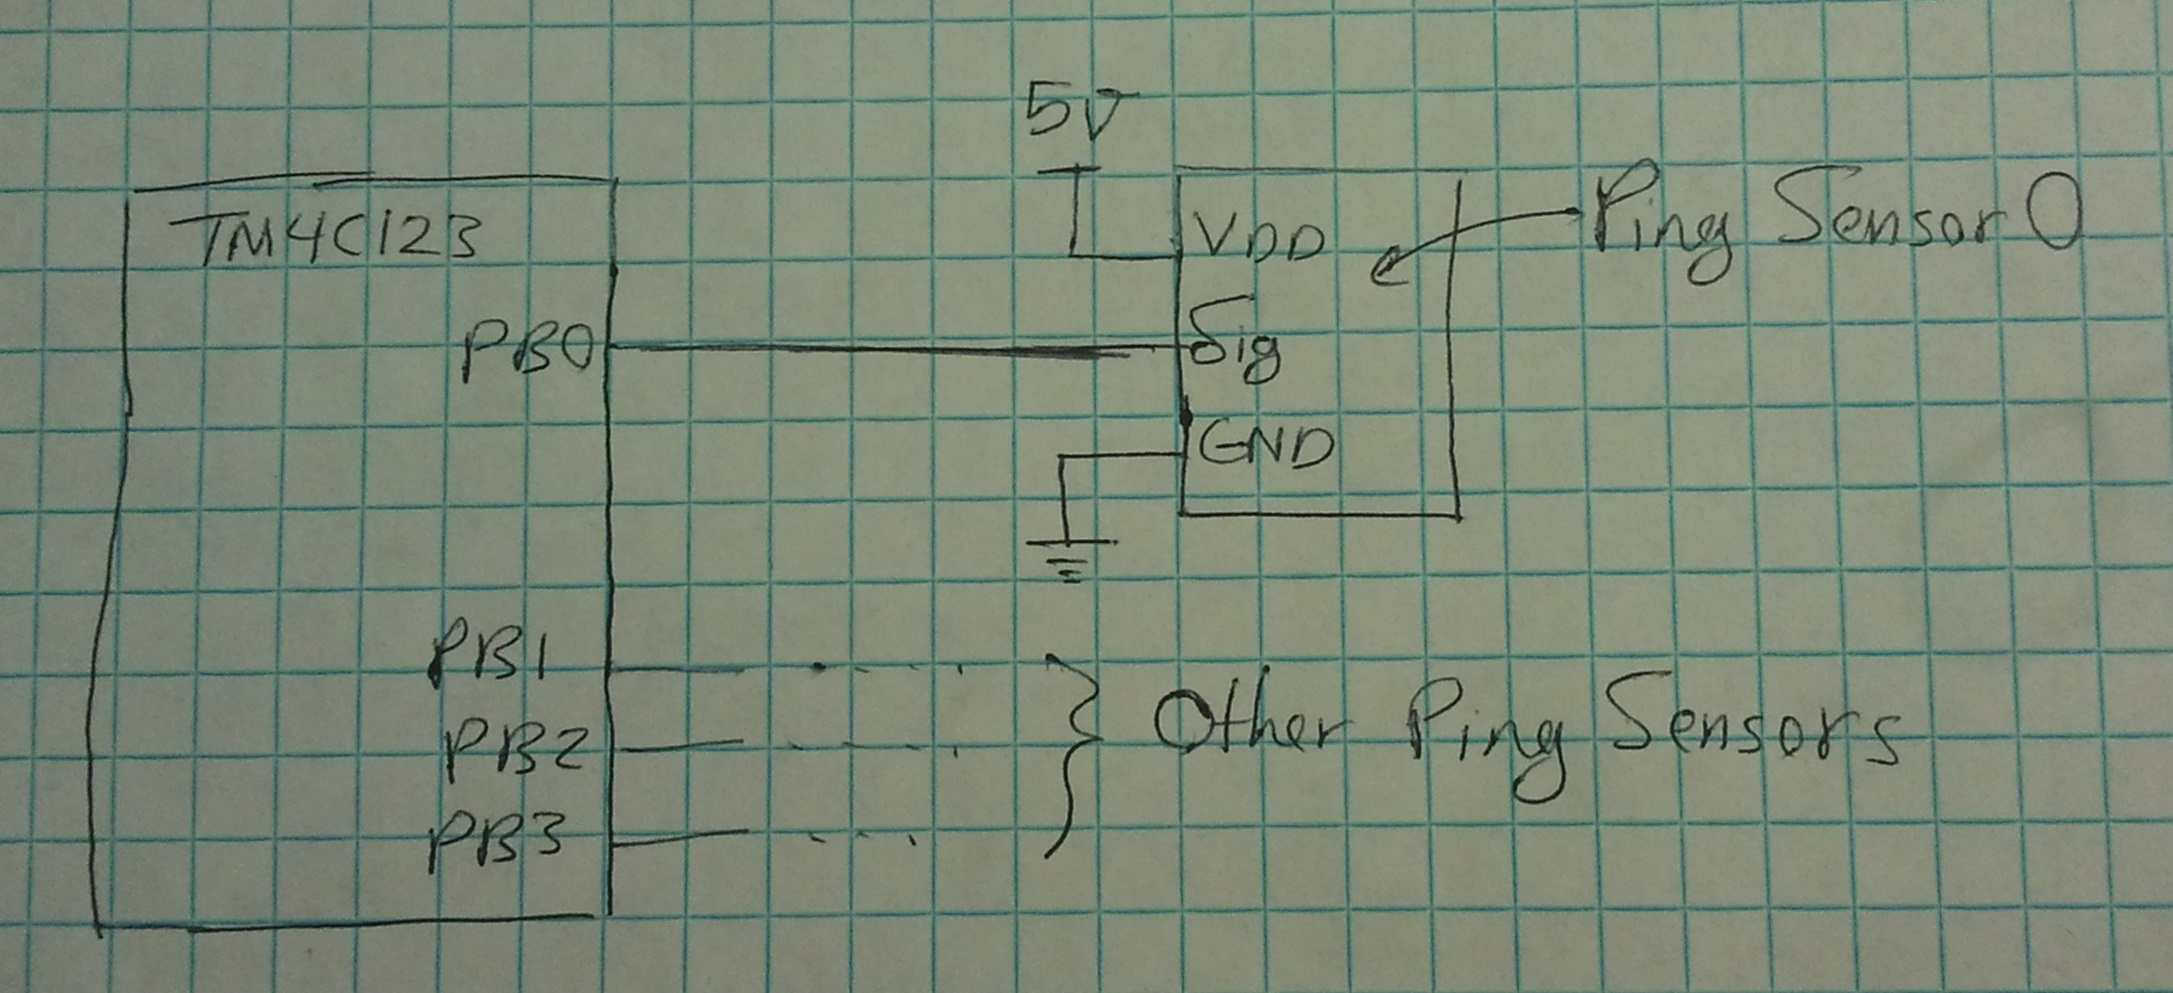
\includegraphics[width=\pic]{circuits/ping}
\caption{Ping Circuit} \label{ping}
\end{figure}

\setlength{\pic}{12cm}
\begin{figure}[htp]
\center
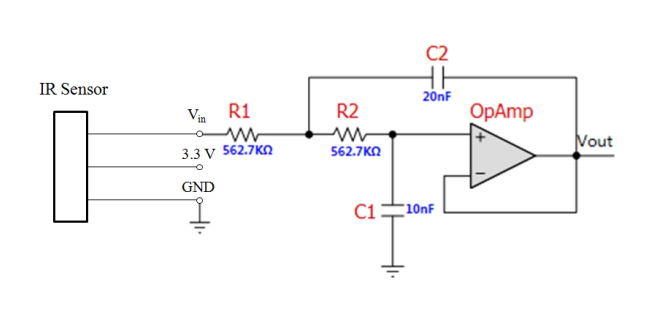
\includegraphics[width=\pic]{circuits/IR_Circuit}
\caption{IR Circuit} \label{ir}
\end{figure}


\section{Software Design}

\lstset{language=C, style=MyCStyle}

\paragraph{(a) Low-level device drivers for the motor interfaces (header and code files) \\}
{
See below
\lstinputlisting{code/motor.h}
\lstinputlisting{code/motor.c}
}

\paragraph{(b) Low-level device drivers for the sensor interfaces (header and code files) \\}
{
IR sensor code is basically the same as Lab.\ 6, but with filter removed. A calibration function is added
that applies linear interpolation to find out the real distance.

\lstinputlisting{code/ir_sensor.h}
\lstinputlisting{code/ir_sensor.c}

The Ping))) sensor code is similar to Lab.\ 6 but now a median filter is added to stabilize the value. Also
the number of sensor is optimized to 2.

\lstinputlisting{code/ping.h}
\lstinputlisting{code/ping.c}

}

\paragraph{(c) High-level competition algorithm \\}
{
Our final competing algorithm employs a PI controller and a finite state machine.

\lstinputlisting{code/algorithm.c}
}

\paragraph{(d) Final data flow graph \\}
See Figure-\ref{df}

\setlength{\pic}{0.8\textwidth}
\begin{figure}[htp]
\center
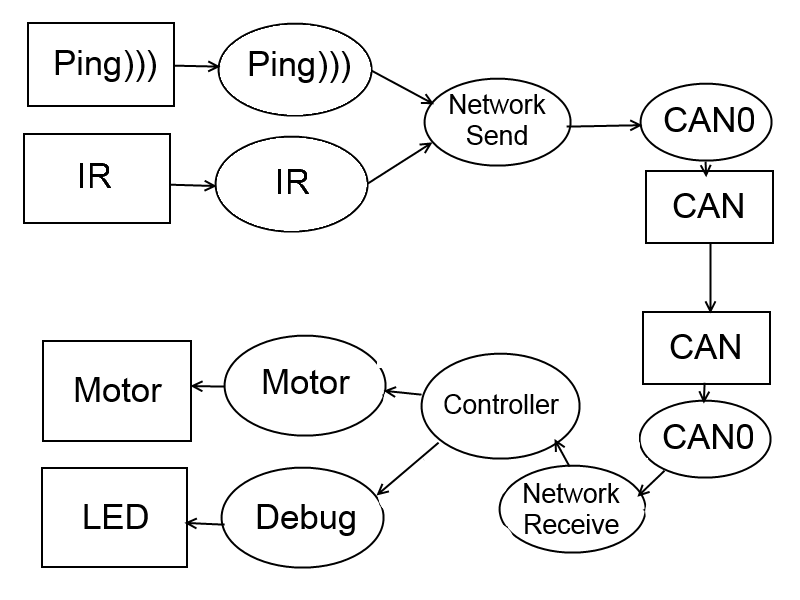
\includegraphics[width=\pic]{pic/dataflow}
\caption{Data flow graph} \label{df}
\end{figure}

\paragraph{(d) Final call graph \\}
See Figure-\ref{cg}

\setlength{\pic}{0.8\textwidth}
\begin{figure}[htp]
\center
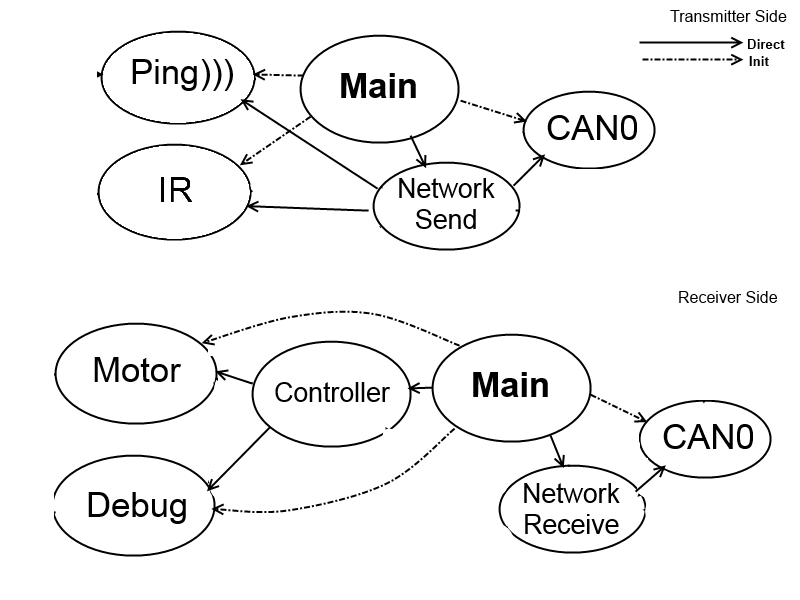
\includegraphics[width=\pic]{pic/callgraph}
\caption{Call graph} \label{cg}
\end{figure}

\section{Measurement}
Our score during the qualification run and final competition is as shown in Table-\ref{tab1}.
\begin{table}
\center
  \begin{tabular}{|c|c|r|}
    \hline
    \multicolumn{3}{|c|}{Scores} \\
    \hline
     Run            & Attempt & Score \\
    \hline
     Qualification  & 1       & 3     \\
                    & 2       & 17    \\
                    & 3       & 8     \\
                    & 4       & 10    \\
    \hline                    
     Competition    & 1       & 15    \\
                    & 2       & 15    \\
                    & 3       & 19    \\                                                         
    \hline
  \end{tabular}
  \caption{Scores}
  \label{tab1}
\end{table}

\newpage
\section{Analysis}
\paragraph{(1) What is the effect of time delay in your control system? \\}
The effect of time delay would be that robot reacts to the environment data that belongs to a previous point in time.
This could result in robot not turning quickly as soon as it finds a gap, the robot not being able to stabilize its
direction among the sides, and the robot hitting the wall before knowing that it has to stop.

\paragraph{(2) What sensors would you need to develop a more effective passing strategy? \\}
IR sensors are more suitable. The most important reason is that IR sensors work well regardless of the angle of the sensor with respective to the object. In this case, since the robot could have any angle to the surrounding walls, IR sensors are the better options compared to ping. Also, IR sensors can provide distance information with lower latency.

\paragraph{(3) If you hit the wall a lot, how could you have changed the design to be more effective? If your robot can 
travel 3 milestones without hitting a wall, you can skip this question. \\}

Our robot passes 3 milestones without hitting a wall.

\paragraph{(4) Briefly explain how odometry could be used in your robot (we discussed it in class). If you used it, how 
well did it work and how could it be improved? If you didn’t use it, why didn’t you use it? \\}

Odometry can be used to estimate the position and orientation of the robot based on its current position. We decided to not use odometry because of two reasons:
\begin{itemize}
\item{First}, odometry requires accurate information of speed and angular velocity. Since we were not using any type of speed sensors, estimating velocity would not result in accurate measurements.
\item{Second}, for the odometry to be effective, an accurate information of the map and environment is required. The prediction of the robot state is not going to be useful if information about the map is not available. 
\end{itemize}


\section{Post-Mortem Team Evaluation}
Here we evaluate the Strengths and Weaknesses by teammate.

\subsection{Chen Cui}
\begin{itemize}
\item[Chen] not obvious in this lab; write code slowly
\item[YKH] Knowledge in C and embedded system; unknown
\item[MQ] perfectionist and experience in C; unknown
\item[Siavash] knowledge and experience; unknown
\item[ZY] knowledge in mechanical and hard-working; unknown
\end{itemize}

\subsection{Yen-Kai Huang}
\begin{itemize}
\item[Chen] Hardworking and experienced in motor interfacing; None
\item[YKH]  Experience in Embedded system and \LaTeX; Not very concentrated
\item[MQ]   Hardworking and easy to work with; Code style is not professional
\item[Siavash] Excellent embedded programmer; He is often busy with the senior design project
\item[ZY]   Very experienced in mechanical engineering and ability of hands-on work ; Lack of embedded experience
\end{itemize}

\subsection{Miao Qi}
\begin{itemize}
\item[Chen]	code is easy readable and in good style, good lab partner; None
\item[YKH]	His code is stylish and easy-readable, strong leadership; None
\item[MQ]	easy to communicate; code is not very portable
\item[Siavash]	Extremely strong coding skill, good organization skill; None
\item[ZY]	hard working, like to explore deeply; None
\end{itemize}

\subsection{Siavash Zangeneh Kamali}
\begin{itemize}
\item[Chen] Hardware interface, embedded systems; Not clear and concise in coding style
\item[YKH] Precise and clear coding style, good at programming, experienced in embedded systems ; Too much perfectionist
\item[MQ] on-time, hard working; Not clear and concise in coding style
\item[Siavash] good at programming, experienced in embedded systems ; Doesn't do things until the deadline is written
\item[ZY] Mechanical engineering stuff, hard working; Not clear and concise in coding style
\end{itemize}

\subsection{Yan Zhang}
\begin{itemize}
\item[Chen] 1. expert in the lab 2. working hard	;	(It's impossible for me to see you guys' weakness...)
\item[YKH]	1. expert in the lab 2. working hard	;	(It's impossible for me to see you guys' weakness...)
\item[MQ]	1. expert in the lab 2. working hard	;	(It's impossible for me to see you guys' weakness...)
\item[Siavash]	1. expert in the lab 2. working hard	;	(It's impossible for me to see you guys' weakness...)
\item[ZY]	1. never give up trying 2. working hard	;	1. little background in EE
\end{itemize}

\subsection*{Failure and Success in Communication}
Thanks to the early set-up with internet tool and code repository, we have had few problems in communication.
An added difficulty surfaces when Nick's cell phone broke and so our smartphone app chatroom can no longer be used
and we had to resort to using Facebook or face-to-face communication more.

\end{document}
